
Before embarking on developing statistical models and generating predictions, it
is essential to understand your data. This is typically done using conventional
numerical and graphical methods. \textcite{tukey1977exploratory} advocated the practice
of exploratory data analysis (EDA) as a critical part of the scientific process.


We present the descriptive statistics of variables in Table
\ref{tab:descriptive-statistic}


\section{Numerical Features}
\label{sec:numerical_features}


\subsection{Price}

The nightly advertised prices range from \$0 to \$10,000. The range is so broad
because hosts do not understand how to set Airbnb advertised prices.  Figure
~\ref{fig:price-distribution-1000} and Figure ~\ref{fig:price-distribution-200}
 show the distributions of price up to \$1,000 and \$200 respectively. While the
price's range is extensive, most of its values concentrate on the range \$10 to
\$1000.  Hence, for minimal values under \$10, we will increase them to \$10,
and values above \$1,000 will be reduced to \$1,000.
\begin{figure}[H]
    %\centering
    \begin{center}

    \caption{Price Distribution}
    \begin{subfigure}[b]{0.48\textwidth}
        \centering
        \caption{Airbnb advertised price up to \$1000}
        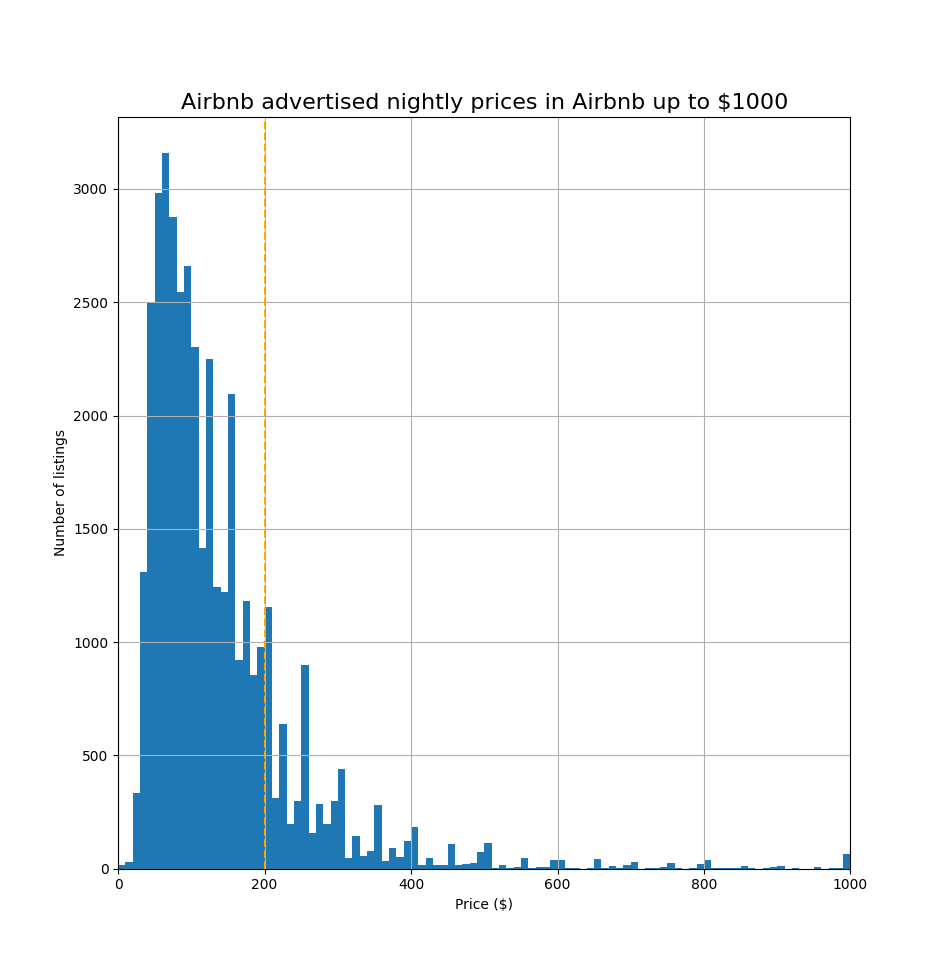
\includegraphics[width=\textwidth]{Figure_6.png}
        \label{fig:price-distribution-1000}
    \end{subfigure}
    \begin{subfigure}[b]{0.48\textwidth}
        \centering
        \caption{Airbnb advertised price up to \$200}
        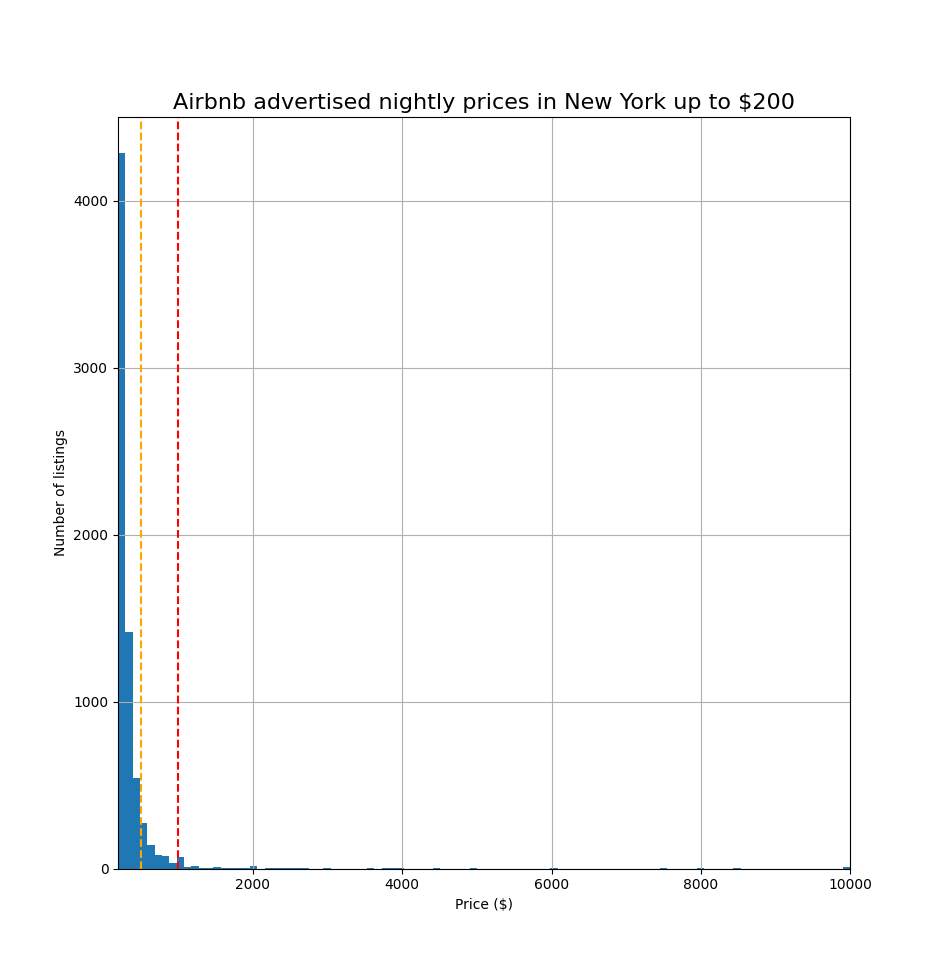
\includegraphics[width=\textwidth]{Figure_7.png}
        \label{fig:price-distribution-200}
    \end{subfigure}

    \end{center}
\end{figure}

\subsection{Host Listings Count}

The median number of listings that the host of each listing has is 1. The mean
is higher (8 in total) due to some hosts own many listings. About 55\% of
listings are from hosts with one listing, and 45\% are from multi-listing hosts.

\subsection{Number of people accommodated, bathrooms, bedrooms and beds}

Figure ~\ref{fig:hist-accommodates} reveals that the most common listing type accommodates two people in
one bed in one bedroom with one bathroom.

\begin{figure}[H] \centering
\caption{Histogram Plot of Accomodate, Bathrooms, Bedrooms, and Beds}
    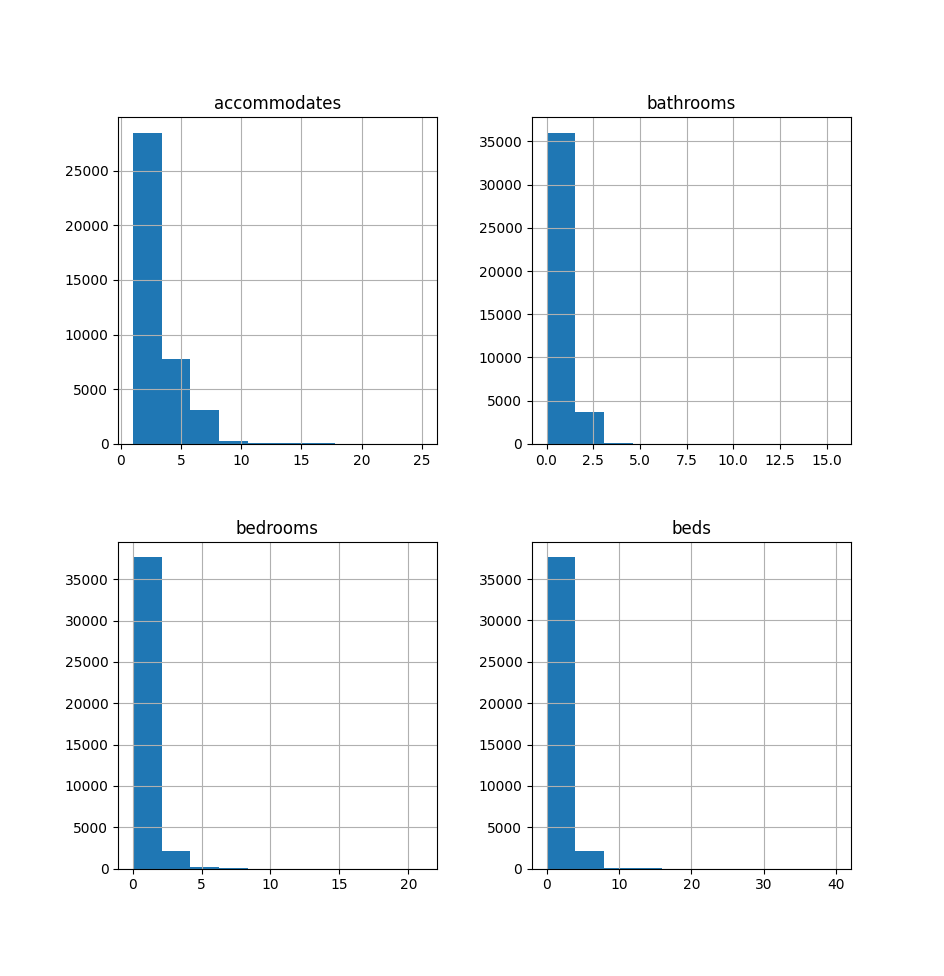
\includegraphics[width=0.75\textwidth]{Figure_9.png}
    \label{fig:hist-accommodates}
\end{figure}

Figure ~\ref{fig:median-price-accommodates} shows that the more people a listing accommodates, the higher the
price they can charge their customers.

\begin{figure}[H] \centering
\caption{Median Price of Airbnb Listing Accommodating Different Number Of Guests}
    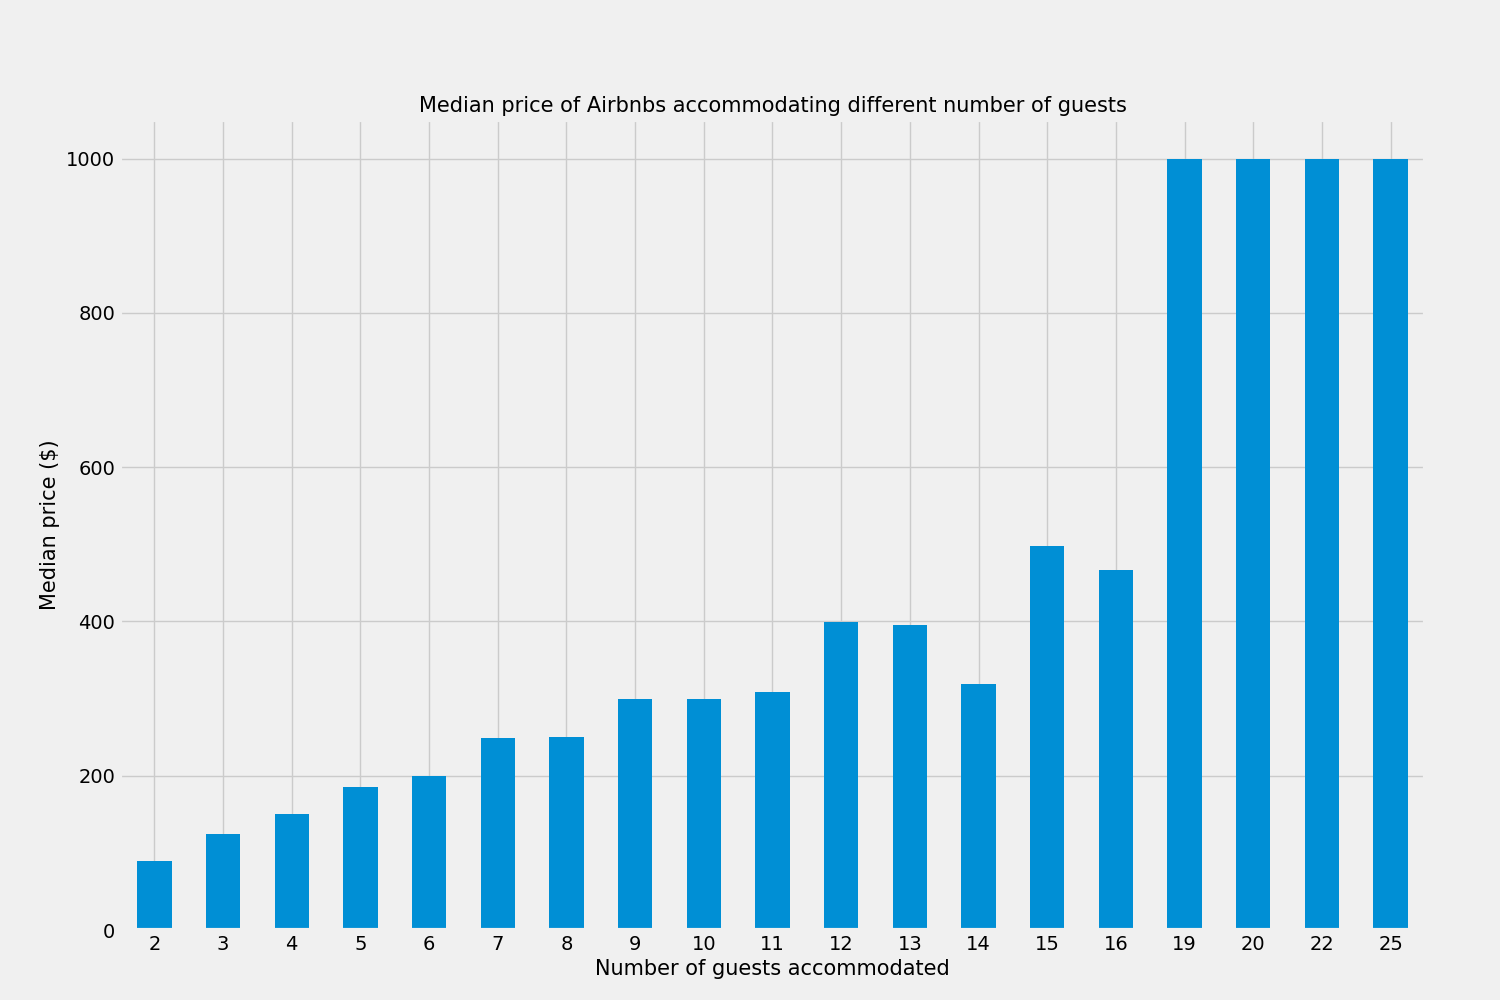
\includegraphics[width=0.75\textwidth]{Figure_8.png}
    \label{fig:median-price-accommodates}
\end{figure}

\section{Categorical features}
\label{sec:categorical_features}

Our main EDA objective for categorical data is to know the unique values and
their corresponding count.

\subsection{Neighbourhood}

Manhattan and Brooklyn have the most Airbnb properties, followed by
Queens (Figure \ref{fig:borough-number-of-listing})
%\begin{figure}[h]\centering
    %\caption{Number of Airbnb listings in each New York borough}
    %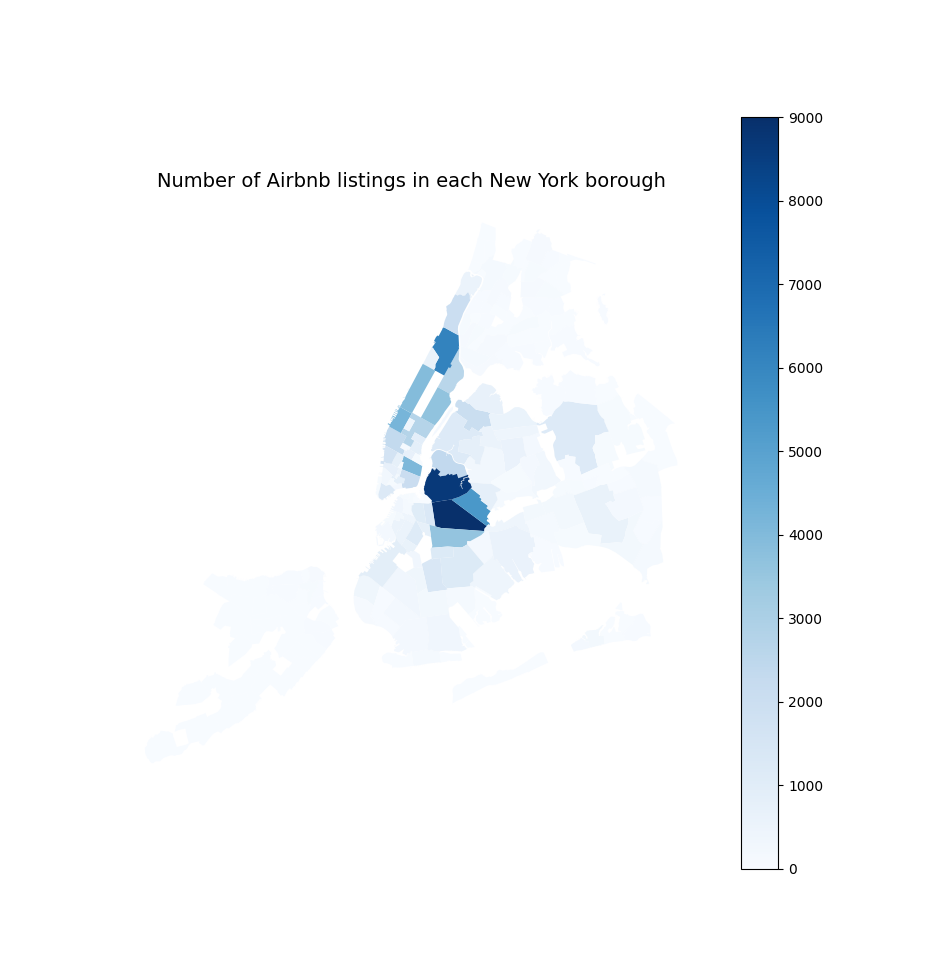
\includegraphics[width=\textwidth]{Figure_10.png}
%\end{figure}
\begin{figure}[H] \centering
\caption{Borough Listings}
    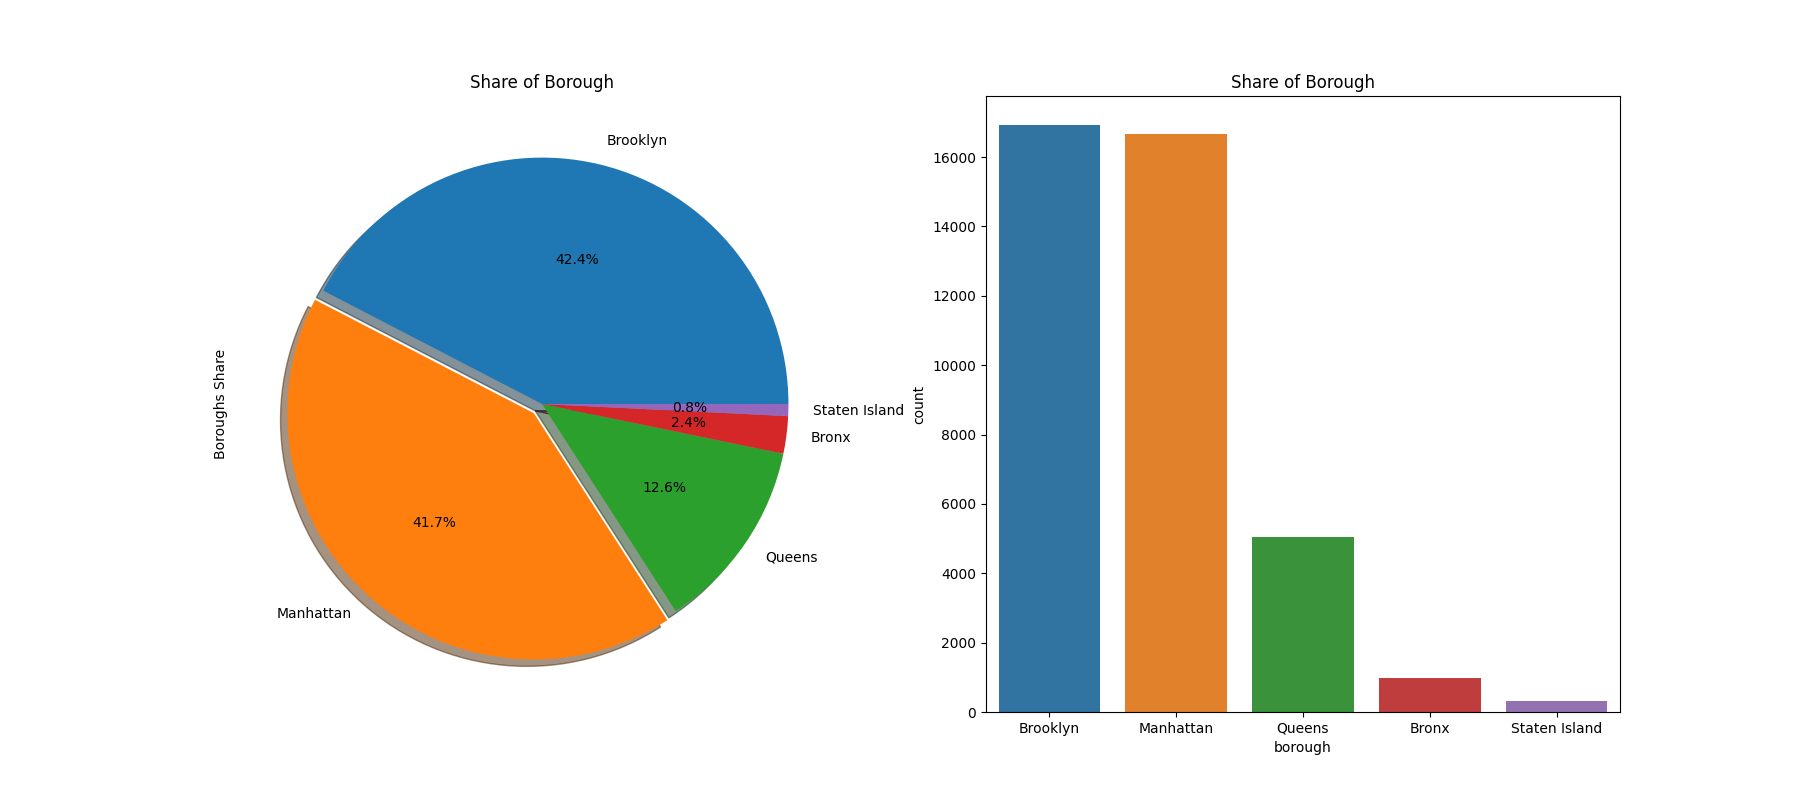
\includegraphics[width=0.75\textwidth]{Figure_10_b.png}
    \label{fig:borough-number-of-listing}
\end{figure}

Top ten neighbourhood with most listings:

\begin{figure}[H] \centering
\caption{Top 10 Neighbourhood with Most Listings}
    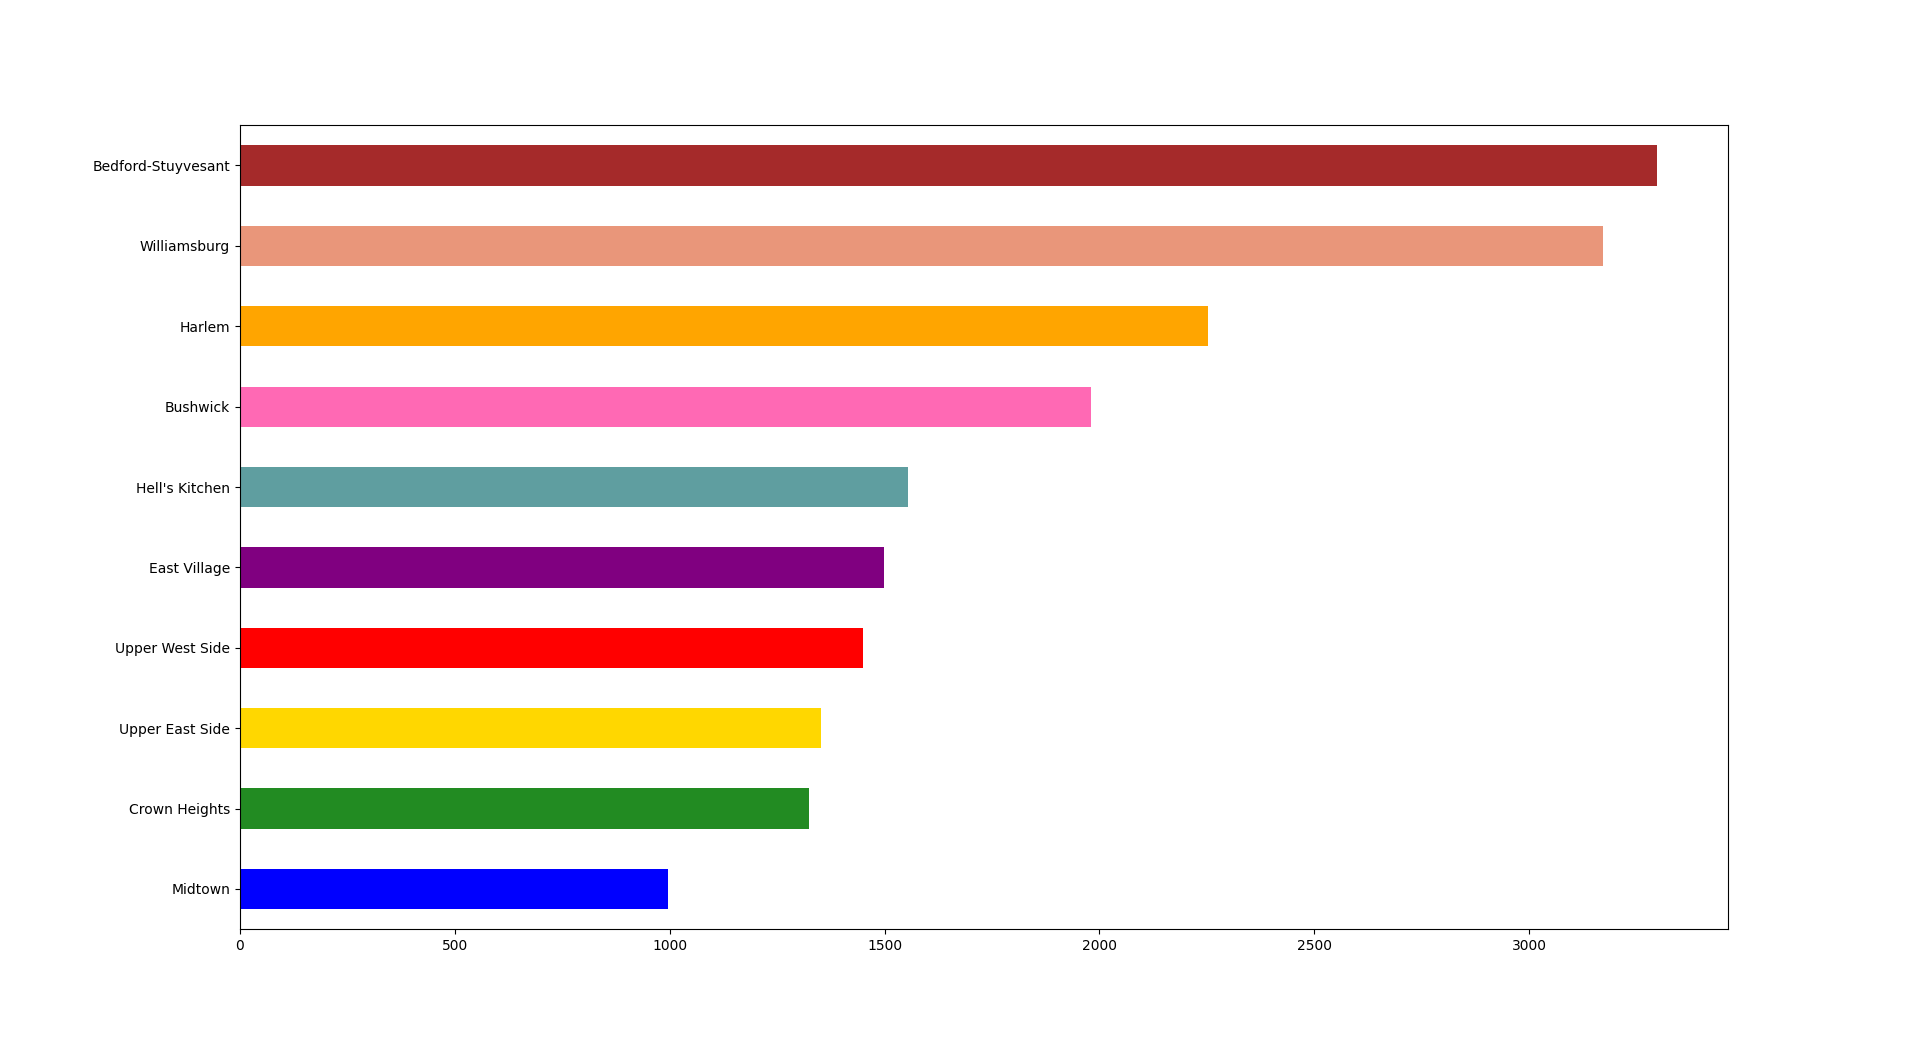
\includegraphics[width=\textwidth]{Figure_10_c.png}
    \label{fig:top-ten-most-listing-neighbourhood}
\end{figure}



As shown in Figure \ref{fig:median-price-borough} and Figure
\ref{fig:borough-price-distribution} , Unsurprisingly, Manhattan is the most
expensive borough - this is a famously expensive area to live, with some of the
world's highest house prices. The second most expensive area is in Brooklyn,
followed by Queens. Staten Island is the least expensive area to rent Airbnb
accommodation.

\begin{figure}[H]\centering
    \caption{Median Price of Airbnb listings in each New York borough}
    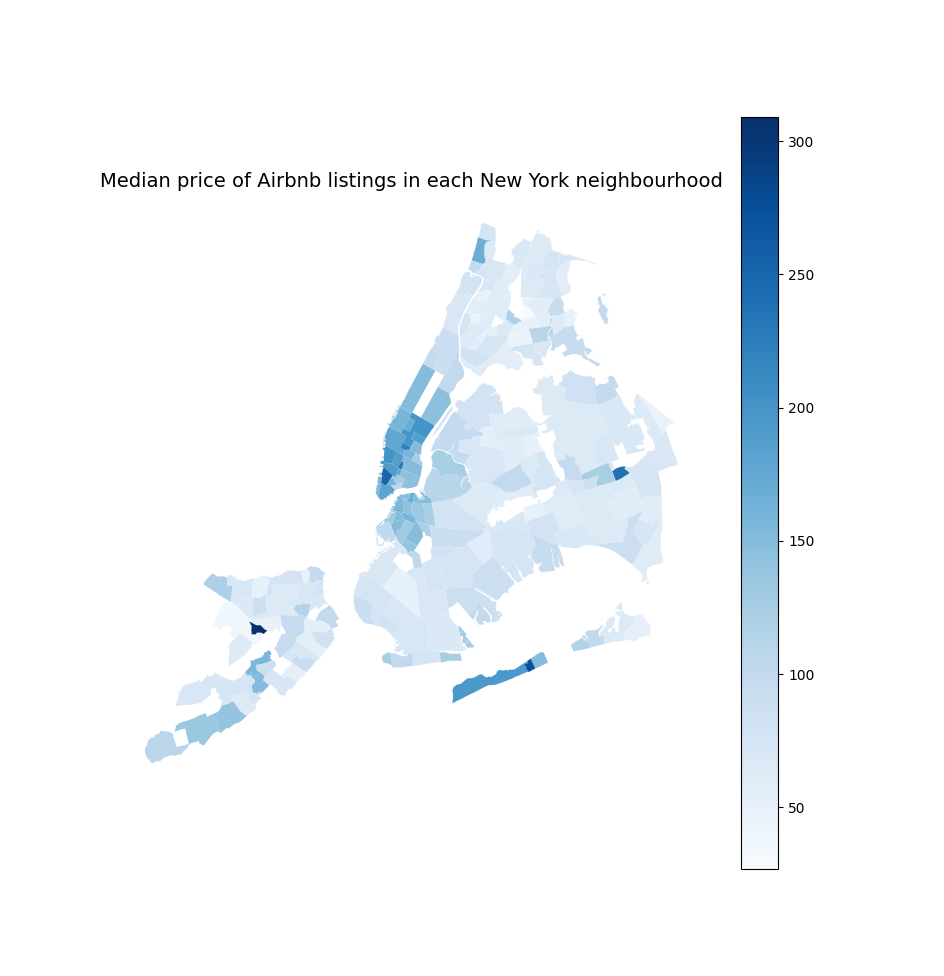
\includegraphics[width=0.75\textwidth]{Figure_11.png}
    \label{fig:median-price-borough}
\end{figure}

\begin{figure}[H]\centering
    \caption{Borough Price Distribution}
    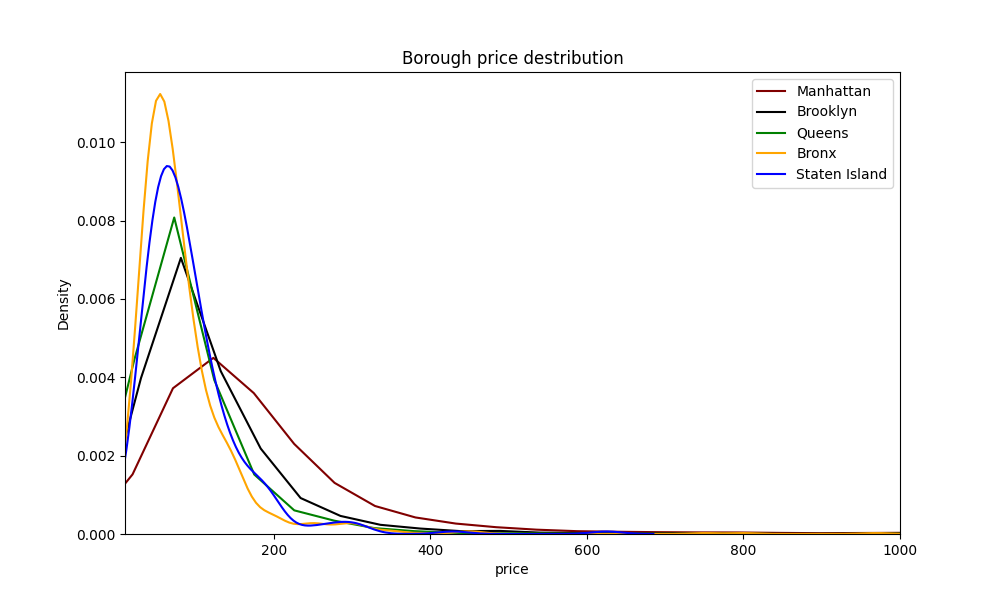
\includegraphics[width=0.75\textwidth]{Figure_11_b.png}
    \label{fig:borough-price-distribution}
\end{figure}

\subsection{Property and room types}

As shown in Figure \ref{fig:property_type},
about 80\% properties are apartments. The remainder are houses or more uncommon
property types (e.g. 'bed and breakfast' or 'yurt').

\begin{figure}[H]
    \centering
    \begin{subfigure}[b]{0.48\textwidth}
        \centering
        \caption{Property Type Pie Chart}
        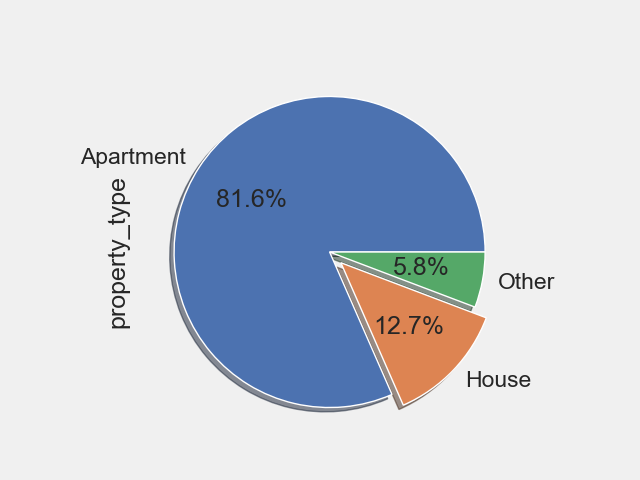
\includegraphics[width=\textwidth]{Figure_12_property_type_pie.png}
        \label{fig:property_type_pie}
    \end{subfigure}
    \begin{subfigure}[b]{0.48\textwidth}
        \centering
        \caption{Property Type Bar Chart}
        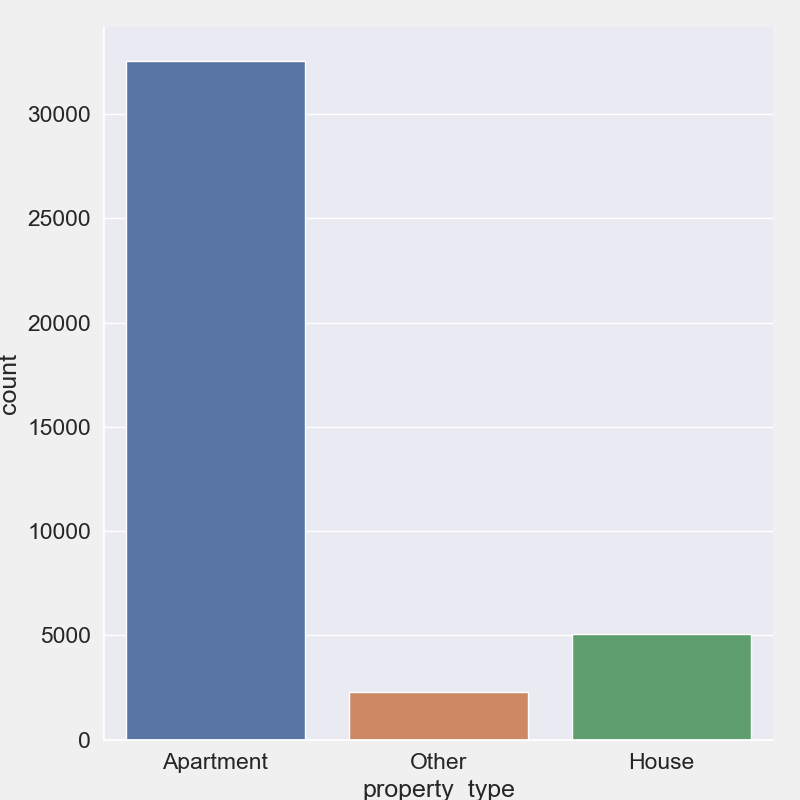
\includegraphics[width=\textwidth]{Figure_12_property_type.png}
        \label{fig:property_type_bar}
    \end{subfigure}

    \caption{Property Type}
    \label{fig:property_type}
\end{figure}

Figure \ref{fig:room_type} shows that about 52\% of listings are entire homes
(i.e. you are renting the entire property on your own). Most of the remainder
are private rooms (i.e. you are renting a bedroom and possibly also a bathroom,
but there will be other people in the property). Fewer than 3\% are shared rooms
(i.e. you are sharing a room with either the property owner or other guests).

\begin{figure}[H]
    \centering
    \begin{subfigure}[b]{0.48\textwidth}
        \centering
        \caption{Room Type Pie Chart}
        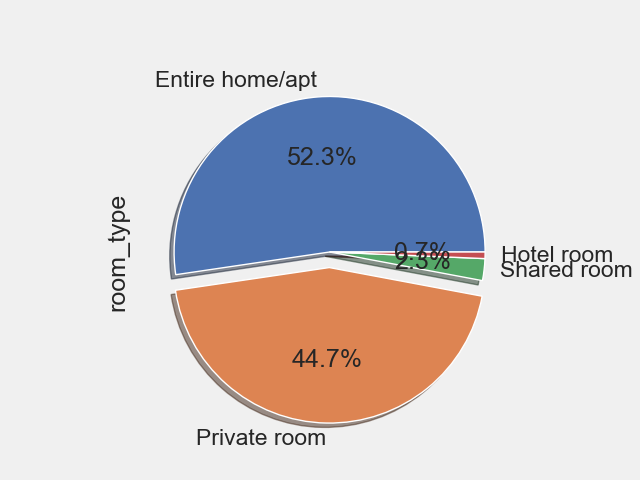
\includegraphics[width=\textwidth]{Figure_12_room_type_pie.png}
        \label{fig:room_type_pie}
    \end{subfigure}
    \begin{subfigure}[b]{0.48\textwidth}
        \centering
        \caption{Room Type Bar Chart}
        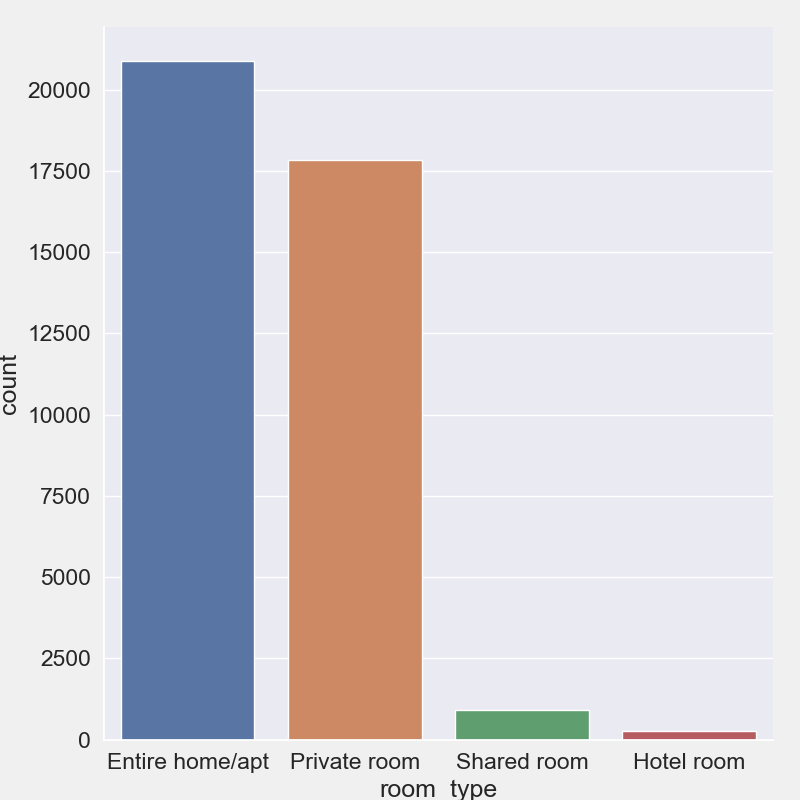
\includegraphics[width=\textwidth]{Figure_12_room_type.png}
        \label{fig:room_type_bar}
    \end{subfigure}
    \caption{Room Type}
    \label{fig:room_type}
\end{figure}

\subsection{Reviews}

From Figure   \ref{fig:overall-listing}, we see that, while few listings receive
review ratings of 80 or below, most listings with a review have received a
95-100/100 overall,  indicating that the customers adore their Airbnbs.

\begin{figure}[H]\centering
    \caption{Overall Listing Rating}
    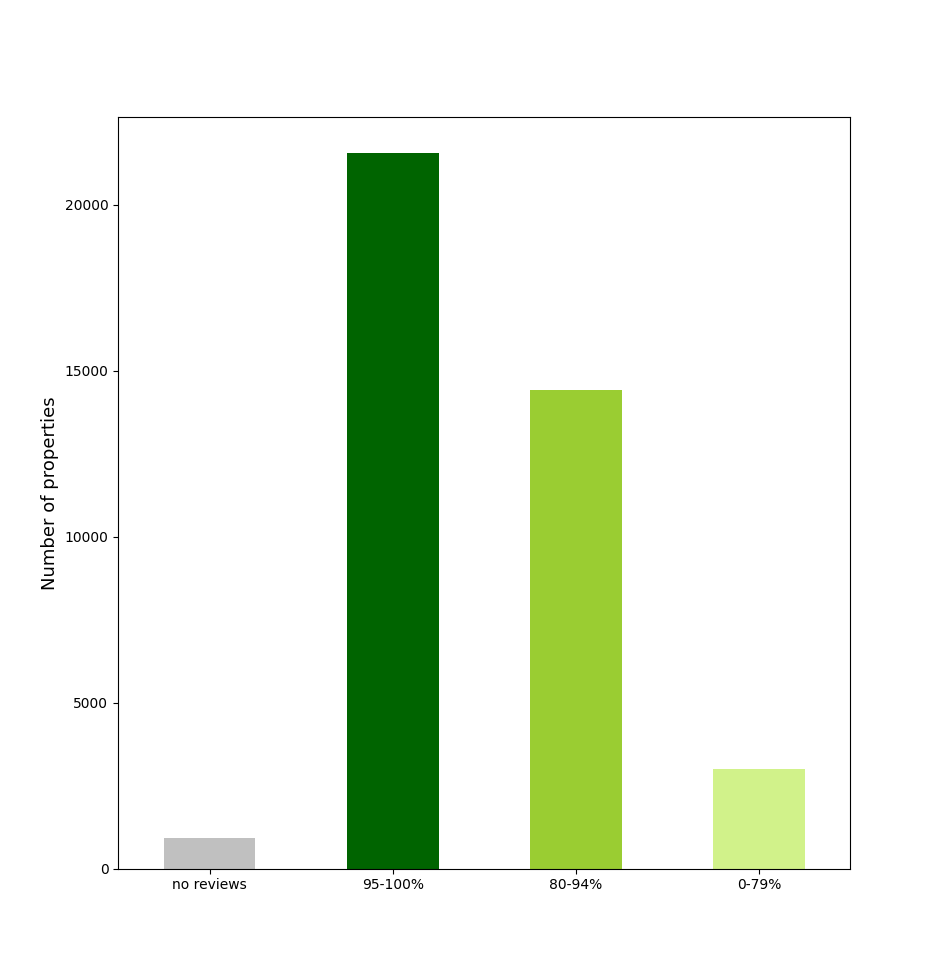
\includegraphics[width=0.75\textwidth]{Figure_13.png}
    \label{fig:overall-listing}
\end{figure}
%Figure \ref{fig:overall-listing-rating}

\subsection{First and Last Review}

As can be seen from the Figure ~\ref{fig:time_since_first_review}, the most
common period in which  Airbnb listings had their first review is 2-3 years,
which means that many listings on the site have been active for at least a
couple of years. However,  fewer listings have been on Airbnb for more than four
years.

The bar plot ~\ref{fig:time_since_last_review} reveals that the most
common period since a listing received its last review is 2-8 weeks, which means
that many listings have been reviewed relatively recently.  What stands out in
the figure is that over 10,000 listings have not had a review for more than a
year, which means they exist on the site, but they do not have their calendars
open and are not available to reserve.

\begin{figure}[H]
    \centering
    \begin{subfigure}[b]{0.48\textwidth}
        \centering
        \caption{Time Since First Review}
        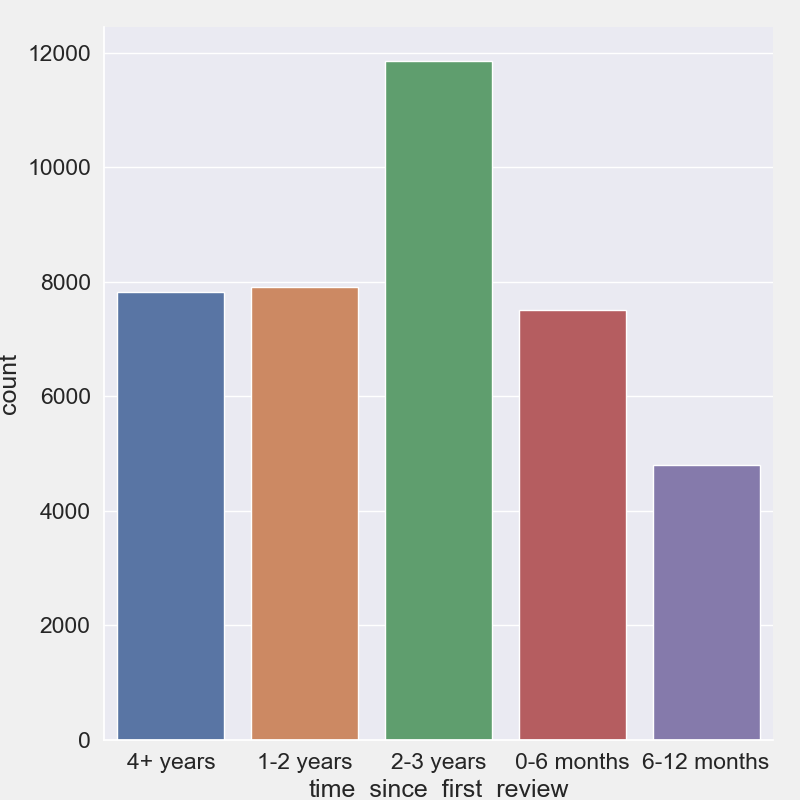
\includegraphics[width=\textwidth]{Figure_15_time_since_first_review.png}
        \label{fig:time_since_first_review}
    \end{subfigure}
    \begin{subfigure}[b]{0.48\textwidth}
        \centering
        \caption{Time Since Last Review}
        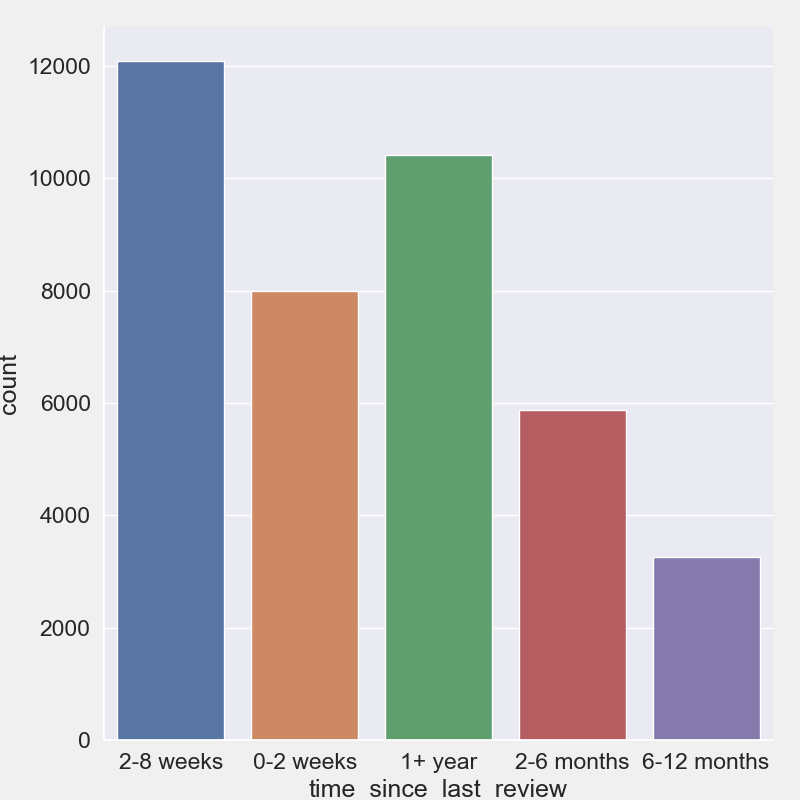
\includegraphics[width=\textwidth]{Figure_15_time_since_last_review.png}
        \label{fig:time_since_last_review}
    \end{subfigure}
    \caption{First and Last Review}
\end{figure}

\section{Boolean features}
\label{sec:boolean_features}

Many features (e.g. for amenities) can be true or false. This section compares
the proportions of these features that are true or false (to explore the data
and also to ascertain whether the feature is worth retaining), and the median
price of each category (to explore the relationship between the category and
price).

\subsection{Superhosts}

Figure ~\ref{fig:host_is_superhost} shows that about 23\% of hosts are "superhosts". As expect that being a superhost (a
mark of quality, requiring various conditions to be met)  improve the median
price of Airbnb listing.

\begin{figure}[H]\centering
    \caption{host\_is\_superhost}
    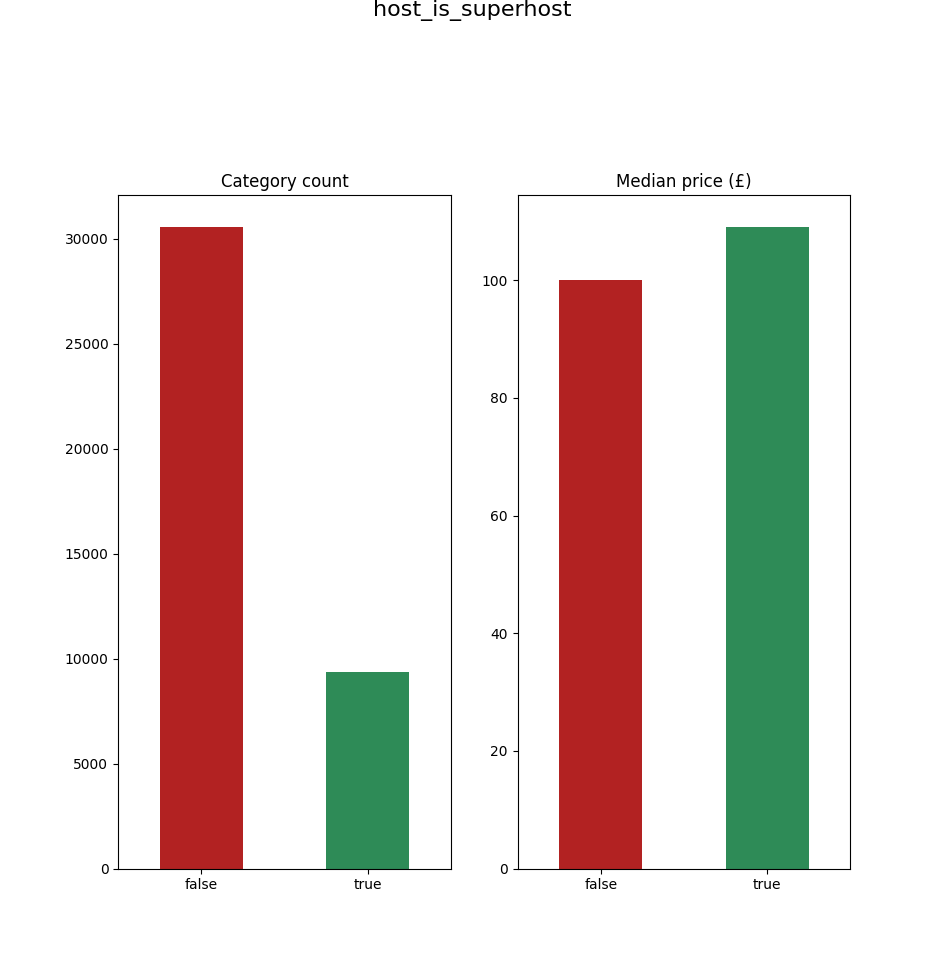
\includegraphics[width=0.75\textwidth]{Figure_16_host_is_superhost.png}
    \label{fig:host_is_superhost}
\end{figure}

\subsection{Host verification}

In Figure ~\ref{fig:host_identity_verified}, about 49\% of hosts are verified.
As with superhost, verifying host's profile (e.g. by providing ID and verifying
your phone number and email address) can lead to a price premium. The reason for
this may have something to do with the fact that providing host's verification
increases the trustworthiness of the host (Ert 2016).

\begin{figure}[H]
    \centering
    \caption{host\_identity\_verified}
    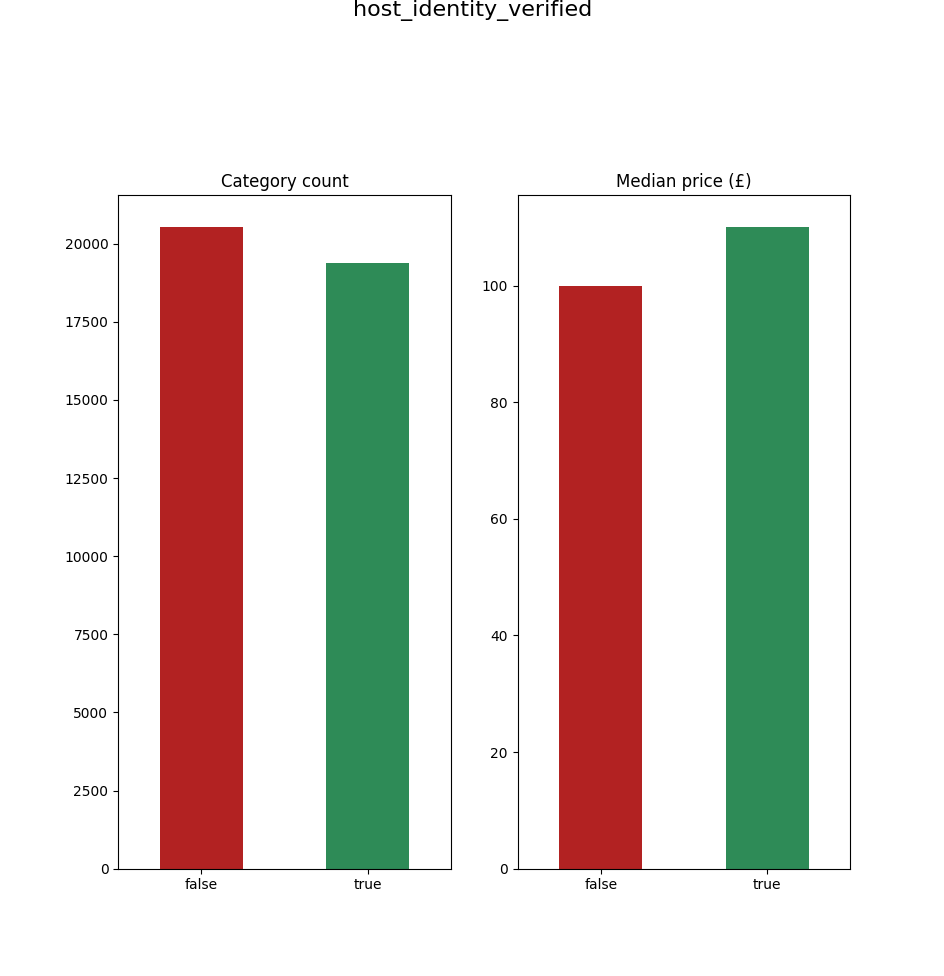
\includegraphics[width=0.75\textwidth]{Figure_16_host_identity_verified.png}
    \label{fig:host_identity_verified}
\end{figure}

\subsection{Instant booking}

As shown in figure below, about 40\% of properties are instant bookable. However, the added
convenience does not seem to have any effect on the median price per night. This
negative link can be explained by both emotional (Wang \& Nicolau 2017) and
economic (Benitez-Aurioles, 2018)

\begin{figure}[H]
    \centering
    \caption{instant\_bookable}
    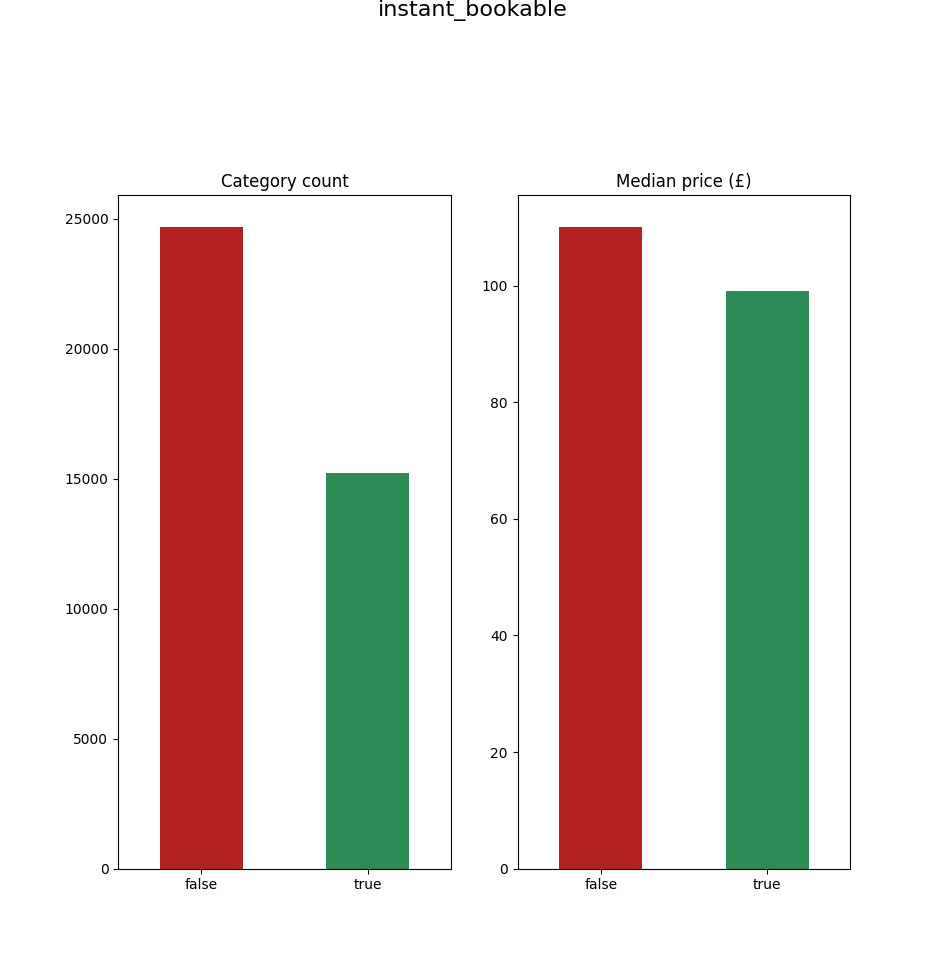
\includegraphics[width=0.75\textwidth]{Figure_16_instant_bookable.png}
    \label{fig:instant_bookable}
\end{figure}

\subsection{Amenities}

Our goal is to identify which amenities are common and which increase the price
of an Airbnb listing.  In Figure ABC, we plot the count plot and each amenity's
median price to explore the relationship between the amenity and price.
Amenities then can be split into three groups:

\begin{enumerate}

  \item The first group contains uncommon amenity, but listings with it have a
    higher median price: Bed linen, Coffee machine, Basic cooking equipment,
    Elevator, Child friendly, Long term stays allowed, Private entrance, Self
check-in, Pets allowed, Air conditioner

  \item The second group includes common amenities and listings with it have a
higher median price: TV, Washer, dryer and/or dishwasher (white goods), Internet

  \item The third group comprises uncommon amenities, and listings with it have
    a lower median price: Parking (presumably because these are less likely to
    be central properties), Greeted by host

\end{enumerate}

%\section{Time Series Analysis}
%\label{sec:time_series}

%Lorem ipsum dolor sit amet, consetetur sadipscing elitr, sed diam nonumy eirmod tempor invidunt ut labore et dolore magna aliquyam erat, sed diam voluptua. At vero eos et accusam et justo duo dolores et ea rebum. Stet clita kasd gubergren, no sea takimata sanctus est Lorem ipsum dolor sit amet.

